\documentclass[a4paper,11pt]{article}
\usepackage{graphicx}
\usepackage{amsmath}
\usepackage{hyperref}
\usepackage{geometry}
\geometry{left=2.5cm,right=2.5cm,top=2.5cm,bottom=2.5cm}

\title{Rapport Jalon 1}
\author{\textbf{Benjamin PELLIEUX}}
\date{\today}

\begin{document}

\maketitle

\section{Problématique Générale}
Dans le cadre de l'optimisation énergétique des bâtiments chauffés par des systèmes à murs radiants en béton, il est primordial de comprendre la répartition de la chaleur dans le matériau. Cette étude vise à modéliser la conduction thermique à travers un mur en béton, un des principaux défis étant de garantir un confort thermique tout en minimisant la consommation énergétique. Les systèmes de chauffage doivent être en mesure de s'adapter aux différentes conditions extérieures et intérieures afin de réduire la consommation d'énergie tout en maintenant une température confortable pour les occupants. Le béton, grâce à sa masse thermique élevée, permet une diffusion de chaleur relativement lente, ce qui en fait un bon candidat pour des systèmes de chauffage intégrés.

\section{Objectifs du Jalon}
Le premier jalon consiste à simuler la conduction thermique stationnaire dans un mur en béton en résolvant le problème à l'aide de la méthode des volumes finis (MVF). L'objectif est de comparer deux types de conditions aux limites :
\begin{itemize}
    \item Condition Dirichlet aux deux extrémités du mur, imposant une température fixe de part et d'autre.
    \item Condition Dirichlet à gauche et condition Neumann à droite, représentant un flux thermique constant.
\end{itemize}
L'objectif est d'observer la répartition de la température à travers le mur dans ces deux configurations.

\section{Méthodologie}
Pour résoudre ce problème, nous utilisons la méthode des volumes finis (MVF) qui permet de discrétiser l'équation de conduction thermique. La méthode consiste à diviser le mur en petits volumes, et à appliquer un bilan d'énergie à chacun d'entre eux. Cette approche est adaptée pour résoudre numériquement des équations différentielles sur des domaines complexes tout en garantissant la conservation de l'énergie.

La discrétisation spatiale est réalisée en découpant le mur en un nombre fini de segments. Nous utilisons ici 1000 volumes pour garantir une bonne précision. La conductivité thermique utilisée pour le béton est de $k = 0.8 \, W/m\cdot K$ \cite{sourceconductivity}, valeur courante pour ce matériau. Le mur a une longueur de 1 mètre, et les conditions aux limites sont définies comme suit :
\begin{itemize}
    \item \textbf{Condition de Dirichlet-Dirichlet} : Température fixe de 100°C à gauche et 25°C à droite.
    \item \textbf{Condition de Dirichlet-Neumann} : Température fixe de 100°C à gauche, et flux thermique nul à droite (Neumann).
\end{itemize}
Aucune considération temporelle n'est prise en compte dans ce jalon car il s'agit d'un régime stationnaire.

\section{Résultats}
Les résultats obtenus montrent la répartition de la température à travers le mur pour les deux configurations de conditions aux limites.

\begin{figure}[h!]
    \centering
    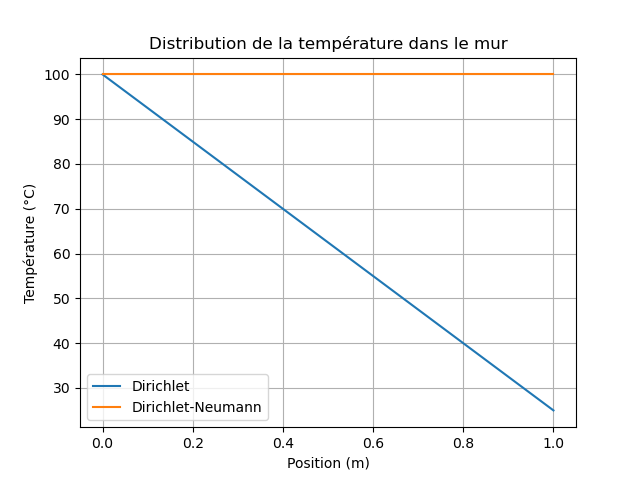
\includegraphics[width=0.8\textwidth]{Figure_1.png}
    \caption{Distribution de la température dans un mur de béton avec conditions Dirichlet et Dirichlet-Neumann.}
    \label{fig:temperature_distribution}
\end{figure}

Comme on peut le voir sur la figure \ref{fig:temperature_distribution}, pour les conditions Dirichlet-Dirichlet, la température diminue de manière quasi-linéaire du côté chaud vers le côté froid. En revanche, avec les conditions Dirichlet-Neumann, la température décroît différemment vers l'extrémité droite, avec un gradient moins prononcé à cause de l'absence de flux thermique sortant à droite (flux nul).

\section{Conclusion}
Les résultats obtenus sont conformes aux attentes théoriques. Le profil de température linéaire observé avec les conditions Dirichlet-Dirichlet correspond à une diffusion de chaleur uniforme dans le mur. Avec la condition Neumann, l'absence de flux thermique à l'extrémité droite perturbe cette diffusion, entraînant un profil de température moins abrupt.

Ce jalon marque l'achèvement de la simulation en régime stationnaire. Le jalon suivant portera sur la simulation de la conduction thermique en régime transitoire, avec un chauffage interne et un contrôle ON/OFF basé sur une température de consigne, ce qui permettra de modéliser des conditions plus réalistes et dynamiques dans les bâtiments.

\begin{thebibliography}{9}
    \bibitem{sourceconductivity} \texttt{https://fr.wikipedia.org/wiki/Liste\_de\_conductivit\%C3\%A9s\_thermiques}, Liste de conductivités thermiques des matériaux.

    \bibitem{sourceconductivity} \texttt{https://materiaux-namur.com/magazine/322/La-conductivite-thermique-des-isolants}, La conductivité thermique des isolants ou le coefficient Lambda.
    \bibitem{} \texttt{https://energieplus-lesite.be/donnees/enveloppe44/enveloppe2/conductivite-thermique-des-materiaux/}, Conductivité thermique des matériaux.
    
\end{thebibliography}

\end{document}

